%%% LaTeX-Vorlage Version 2.1 %%%

% TODO: individuelle Einstellungen (Name, Titel etc.)
% -> bitte in Konfigurationsdatei anpassen
%%%%
%
% Zentrale Konfigurationsdatei
%
% In dieser Datei sind eine Reihe verpflichtender Einstellungen 
% (Nr. 1 bis 6) vorzunehmen.
%
% Die Einstellungen unter Nr. 7 bis 11 können im Regelfall unverändert
% belassen werden. Ausnahmen sind:
%  - Ihre Arbeit ist in englischer Sprache verfasst (Nr. 7)
%  - der Titel Ihrer Arbeit ist sehr lang, so dass er nicht auf das
%    Deckblatt passt oder anders umgebrochen werden soll (Nr. 8 und 9)
%  - es soll ein besonderes Abgabedatum angegeben werden (Nr. 10)
%  - Sie benötigen einen Vertraulichkeitsvermerk (Nr. 11)
%
%%%%


% TODO 1. Typ der Arbeit (für Titelseite und Metadaten)
% Zutreffendes auswählen:

\newcommand{\typMeinerArbeit}{Projektarbeit T2000} 
%\newcommand{\typMeinerArbeit}{PA1} 
%\newcommand{\typMeinerArbeit}{PA2} 
%\newcommand{\typMeinerArbeit}{Seminararbeit} 
%\newcommand{\typMeinerArbeit}{BA} 

% TODO 2. Vorname, Name der Autorin/des Autors (für Deckblatt und Metadaten)
\newcommand{\meinName}{Tudor Lupsa}

% TODO 3. Kurs eintragen
\newcommand{\meinKurs}{xxx}

% TODO 4. Titel der Arbeit (für Deckblatt, ehrenwörtliche Erklärung und Metadaten, ohne Umbrüche angeben)
\newcommand{\themaMeinerArbeit}{Mein Titel}

% TODO 5. Angaben zum Unternehmen (wird bei Seminararbeiten nicht angezeigt)
\newcommand{\UNName}{Firma XY}
\newcommand{\UNBetreuer}{Titel, Vorname und Nachname}
\newcommand{\UNBetreuerFunktion}{Funktion des Betreuers/der Betreuerin}

% TODO 6. Angaben zur wissenschaftlichen Betreuung 
\newcommand{\DHBWBetreuer}{Titel, Vorname und Nachname}


% OPTIONALE Einstellungen

% 7. Arbeit in Englisch
% (nur ändern, falls Ihre Arbeit in englischer Sprache geschrieben ist)
\newcommand{\meineSprache}{DE}	% Standard-Einstellung
%\newcommand{\meineSprache}{EN}	% für Arbeiten in englischer Sprache

% 8. Schriftgröße des Titels auf Deckblatt
% (nur ändern, falls Sie einen sehr langen Titel haben)
% Zutreffendes auswählen:
\newcommand{\schriftgroesseTitel}{\LARGE}   % Standard-Einstellung
%\newcommand{\schriftgroesseTitel}{\Large}  % bei sehr langen Titeln

% 9. Titel mit Umbrüchen für Deckblatt
% (nur ändern, falls Sie den Zeilenumbruch selbst beeinflussen möchten)
\newcommand{\titelAufDeckblatt}{\themaMeinerArbeit}		% Standard-Einstellung
%\newcommand{\titelAufDeckblatt}{Herausforderungen der Digitalisierung im globalen Wettbewerb von Industrieunternehmen \\ -- eine vergleichende Untersuchung unter Berücksichtigung aktueller und weniger aktueller Forschungsmethoden \\ am Beispiel der Firma Melanie Müller und Söhne AG} % explizite Angabe

% 10. Abgabedatum anpassen
% Zutreffendes auswählen:
\newcommand{\abgabeDatum}{\today}  		% Standard-Einstellung
%\newcommand{\abgabeDatum}{TT.MM.JJJJ}  % falls nicht aktuelles Datum

% 11. Vertraulichkeitsvermerk
% (nur ändern, falls Ihre Arbeit einen Vertraulichkeitsvermerk tragen soll)
\newcommand{\hatVermerk}{nein}  	% Standard-Einstellung
% \newcommand{\hatVermerk}{ja}  	% falls Vertraulichkeitsvermerk



% Grundlegende Dokumenteneigenschaften gemäß DHBW-Vorgaben
\documentclass[a4paper,fontsize=11pt,oneside,parskip=half,headings=normal,listof=nochaptergap]{scrreprt} 
% \usepackage{showframe} % nur für Kontrolle der Ränder 

%%% Präambel einbinden (mit Festlegungen gemäß DHBW-Vorgaben) %%%
%%% Präambel %%%
% Sprachumschaltung DE/EN
\usepackage{ifthen}
\newcommand{\DEoEN}[2]{\ifthenelse{\equal{\meineSprache}{DE}}{#1}{#2}}

% Zeichencodierung/Fonts
\usepackage[utf8]{inputenc}
\usepackage[T1]{fontenc}

% Farben + Code-Listings
\usepackage{xcolor}      % statt 'color' (mehr Features)
\usepackage{listings}
% Grund-Setup für Listings (Umlaute/EUR etc.)
\lstset{numbers=left, numberstyle=\tiny, numbersep=5pt, texcl=true}
\lstset{literate=
{Ö}{{\"O}}1 {Ä}{{\"A}}1 {Ü}{{\"U}}1 {ß}{{\ss}}2
{ü}{{\"u}}1 {ä}{{\"a}}1 {ö}{{\"o}}1 {€}{{\euro}}1
}
% Lesbares Listing-Layout + automatischer Zeilenumbruch
\lstdefinestyle{code}{
  numbers=left, numberstyle=\tiny, numbersep=5pt,
  breaklines=true, breakatwhitespace=true,
  columns=fullflexible, keepspaces=true, tabsize=2,
  basicstyle=\ttfamily\small,
  postbreak=\mbox{\textcolor{gray}{$\hookrightarrow$}}\space
}
\lstset{style=code}

% Seitenränder
\usepackage[
  left=2.5cm, right=2.5cm,
  top=2.5cm, bottom=2.5cm,
  foot=12mm, includefoot
]{geometry}

% Sprache + Anführungszeichen
\DEoEN{
  \usepackage[ngerman]{babel}
  \usepackage[babel,german=quotes]{csquotes}
}{
  \usepackage[english]{babel}
  \usepackage[babel,english=british]{csquotes}
}

% Listen, Grafiken, Zeilenabstand
\usepackage{enumerate}
\usepackage{graphicx}
\graphicspath{{img/}}
\usepackage[onehalfspacing]{setspace}

% Testtext, Akronyme
\usepackage{blindtext}
% \usepackage{color}  % durch xcolor ersetzt
\usepackage[nohyperlinks]{acronym}

% Literatur (biblatex + DHBW-Config)
\usepackage[
  backend=biber,
  bibstyle=_dhbw_authoryear,maxbibnames=99,
  citestyle=authoryear, dashed=false,
  uniquename=true, useprefix=true,
  bibencoding=utf8
]{biblatex}
%kein Punkt am Ende bei \footcite
%http://www.golatex.de/footcite-ohne-punkt-am-schluss-t4865.html
\renewcommand{\bibfootnotewrapper}[1]{\bibsentence#1}

% Bibliographie: Vornamen ausgeschrieben
\DeclareNameAlias{author}{family-given}
\DeclareNameAlias{editor}{family-given}

%Reihenfolge der Autorennamen
%   
% http://golatex.de/viewtopic,p,80448.html#80448
% Argumente: siehe http://texwelt.de/blog/modifizieren-eines-biblatex-stils/
\DeclareNameFormat{sortname}{% Bibliographie
  \ifnum\value{uniquename}=0 % Normalfall
    \ifuseprefix%
      {%
         \usebibmacro{name:family-given}
           {\namepartfamily}
           {\namepartgiveni}
           {\namepartprefix}
           {\namepartsuffixi}%
       }
      {%
         \usebibmacro{name:family-given}
           {\namepartfamily}
           {\namepartgiveni}
           {\namepartprefixi}
           {\namepartsuffixi}%
       }%
  \fi
  \ifnum\value{uniquename}=1% falls nicht eindeutig, abgek. Vorname 
      {%
         \usebibmacro{name:family-given}
           {\namepartfamily}
           {\namepartgiveni}
           {\namepartprefix}
           {\namepartsuffix}%
       }%
  \fi
  \ifnum\value{uniquename}=2% falls nicht eindeutig, ganzer Vorname 
      {%
         \usebibmacro{name:family-given}
           {\namepartfamily}
           {\namepartgiven}
           {\namepartprefix}
           {\namepartsuffix}%
       }%
  \fi   
  \usebibmacro{name:andothers}}

\DeclareNameFormat{labelname}{% für Zitate
  \ifnum\value{uniquename}=0 % Normalfall
    \ifuseprefix%
      {%
         \usebibmacro{name:family-given}
           {\namepartfamily}
           {\empty}
           {\namepartprefix}
           {\namepartsuffixi}%
       }
      {%
         \usebibmacro{name:family-given}
           {\namepartfamily}
           {\empty}
           {\namepartprefixi}
           {\namepartsuffixi}%
       }%
  \fi
  \ifnum\value{uniquename}=1% falls nicht eindeutig, abgek. Vorname 
      {%
         \usebibmacro{name:family-given}
           {\namepartfamily}
           {\namepartgiveni}
           {\namepartprefix}
           {\namepartsuffix}%
       }%
  \fi
  \ifnum\value{uniquename}=2% falls nicht eindeutig, ganzer Vorname 
      {%
         \usebibmacro{name:family-given}
           {\namepartfamily}
           {\namepartgiven}
           {\namepartprefix}
           {\namepartsuffix}%
       }%
  \fi   
  \usebibmacro{name:andothers}}
      
  
\DeclareFieldFormat{extrayear}{% = the 'a' in 'Jones 1995a'
  \iffieldnums{labelyear}
    {\mknumalph{#1}}
    {\mknumalph{#1}}}        

% Namen getrennt durch Komma (Zitate)
\DeclareDelimFormat*[footcite,cite,textcite,parencite]{multinamedelim}{\addcomma\space}
% bzw. Semikolon (Literaturverzeichnis)
\DeclareDelimFormat[bib,biblist]{multinamedelim}{\addsemicolon\space}
% keine besondere Behandlung beim letzten Autor
\DeclareDelimAlias{finalnamedelim}{multinamedelim}
%\DeclareDelimAlias{multilistdelim}{multinamedelim}

\renewcommand{\nameyeardelim}{~}

% Literaturverzeichnis: Doppelpunkt zwischen Name (Jahr): Rest 
% http://de.comp.text.tex.narkive.com/Tn1HUIXB/biblatex-authoryear-und-doppelpunkt
\renewcommand{\labelnamepunct}{\addcolon\addspace}

% damit die Darstellung für Vollzitate von Primärquellen in 
% Fußnoten später auf "nicht fett" geändert werden kann 
% (nur für Zitate von Sekundärliteratur relevant)
\newcommand{\textfett}[1]{\textbf{#1}}

% für Zitate von Sekundärliteratur:
\newcommand{\footcitePrimaerSekundaer}[4]{%
  \renewcommand{\textfett}[1]{##1}%
  \footnote{\fullcite[#2]{#1}, \DEoEN{zitiert nach}{as cited in} \cite[#4]{#3}}%  
  \renewcommand{\textfett}[1]{\textbf{##1}}%
}

% Im Literaturverzeichnis: Autor (Jahr) fett
\renewbibmacro*{author}{%
  \ifboolexpr{%
    test \ifuseauthor%
    and
    not test {\ifnameundef{author}}
  }
    {\usebibmacro{bbx:dashcheck}
       {\bibnamedash}
       {\usebibmacro{bbx:savehash}%
        \textfett{\printnames{author}}%
        \iffieldundef{authortype}
          {\setunit{\addspace}}
          {\setunit{\addcomma\space}}}%
     \iffieldundef{authortype}
       {}
       {\usebibmacro{authorstrg}%
        \setunit{\addspace}}}%
    {\global\undef\bbx@lasthash
     \usebibmacro{labeltitle}%
     \setunit*{\addspace}}%
  \textfett{\usebibmacro{date+extrayear}}}

% Sonderfall: Quelle ohne Autor, aber mit Herausgeber
% Name des Herausgebers wird fett gedruckt
\renewbibmacro*{bbx:editor}[1]{%
  \ifboolexpr{%
    test \ifuseeditor%
    and
    not test {\ifnameundef{editor}}
  }
    {\usebibmacro{bbx:dashcheck}
       {\bibnamedash}
       {\textfett{\printnames{editor}}%
        \setunit{\addcomma\space}%
        \usebibmacro{bbx:savehash}}%
     \usebibmacro{#1}%
     \clearname{editor}%
     \setunit{\addspace}}%
    {\global\undef\bbx@lasthash
     \usebibmacro{labeltitle}%
     \setunit*{\addspace}}%
  \textfett{\usebibmacro{date+extrayear}}}

\DefineBibliographyStrings{ngerman}{% Anpassungen für deutsche Sprache
	nodate = {{o.J.}},
	urlseen = {{Abruf:}},
	ibidem = {{ebenda}},
	andothers = {{et\addabbrvspace al\adddot}}
}
\DefineBibliographyStrings{english}{% Anpassungen für englische Sprache
    nodate = {{w.y.}},
    urlseen = {{retrieval:}}
}

% keine Anführungszeichen beim Titel im Literaturverzeichnis
\DeclareFieldFormat[article,book,inbook,inproceedings,manual,misc,phdthesis,thesis,online,report]{title}{#1\isdot}

\newcommand{\literaturverzeichnis}{%
% nur Literaturverzeichnis
% (als eigenes Kapitel)
\phantomsection
\addcontentsline{toc}{chapter}{\refname}
\spezialkopfzeile{\refname}
\defbibheading{lit}{\chapter*{\refname}}
\label{chapter:quellen}
\printbibliography[heading=lit,notkeyword=ausblenden]
}


% Verzeichnisse/Tabellen
\usepackage{tocloft}
\usepackage{multirow}
\usepackage{amsmath}
\usepackage{amssymb}
\usepackage{booktabs}

% Hyperlinks
\usepackage[hypertexnames=false]{hyperref}

% Bessere Umbrüche in \url{…}
\usepackage{xurl}
\urlstyle{tt}

% Intelligente Referenzen (nach hyperref laden!)
\usepackage[capitalise,nameinlink,noabbrev]{cleveref}
% "Listing" -> "Quellcode" (auch für Verzeichnis und Verweise)
\renewcommand{\lstlistingname}{Quellcode}
\renewcommand{\lstlistlistingname}{Quellcodeverzeichnis}
\providecommand*{\lstlistingautorefname}{Quellcode}
\crefname{lstlisting}{Quellcode}{Quellcode}
\Crefname{lstlisting}{Quellcode}{Quellcode}

% Anhangszähler/Verzeichnis (wie in deiner Vorlage)
\newcounter{anhcnt}\setcounter{anhcnt}{0}
\newlistof{anhang}{app}{}
\newcommand{\anhang}[1]{%
  \refstepcounter{anhcnt}\setcounter{anhteilcnt}{0}
  \section*{\appendixname\ \theanhcnt: #1}
  \addcontentsline{app}{section}{\protect\numberline{\appendixname\ \theanhcnt}#1}\par
}
\newcounter{anhteilcnt}\setcounter{anhteilcnt}{0}
\newcommand{\anhangteil}[1]{%
  \refstepcounter{anhteilcnt}
  \subsection*{\appendixname\ \arabic{anhcnt}/\arabic{anhteilcnt}: #1}
  \addcontentsline{app}{subsection}{\protect\numberline{\appendixname\ \theanhcnt/\arabic{anhteilcnt}}#1}\par
}
\renewcommand{\theanhteilcnt}{\appendixname\ \theanhcnt/\arabic{anhteilcnt}}

% tocloft-Einrückungen für Anhangverzeichnis
\makeatletter
\newcommand{\abstaendeanhangverzeichnis}{%
  \renewcommand*{\l@section}{\@dottedtocline{1}{0em}{5.5em}}
  \renewcommand*{\l@subsection}{\@dottedtocline{2}{2.3em}{6.5em}}
}
% Einträge LOF/LOT und Quellcodeverzeichnis (LOL) angeglichen
\renewcommand*{\l@figure}{\@dottedtocline{1}{0em}{2.3em}}
\renewcommand*{\l@table}{\@dottedtocline{1}{0em}{2.3em}}
\renewcommand*{\l@lstlisting}{\@dottedtocline{1}{0em}{2.3em}}
\makeatother

% Fortlaufende Zähler über Kapitel hinweg
\usepackage{chngcntr}
\counterwithout{figure}{chapter}
\counterwithout{table}{chapter}
\counterwithout{footnote}{chapter}

% Kopfzeilen (KOMA-Script)
\usepackage[automark]{scrlayer-scrpage}
%% Definitionen für Kopf- und Fußzeile auf normalen Seiten
\defpagestyle{kopfzeile}
{% Kopfdefinition
  (\textwidth,0pt)    % Länge der oberen Linie,Dicke der oberen Linie       
  {} % Definition für linke Seiten im doppelseitigen Layout
  {} % Definition für rechte Seiten im doppelseitigen Layout      
  {  % Definition für Seiten im einseitigen Layout
	\makebox[0pt][l]{\rightmark}% 
	\makebox[\linewidth]{}% 
  }        
  (\textwidth, 0.4pt) % Untere Linienlänge, Untere Liniendicke
}
{% Fußdefinition
  (\textwidth,0pt)    % Obere Linienlänge, Obere Liniendicke
  {} % Definition für linke Seiten im doppelseitigen Layout
  {} % Definition für rechte Seiten im doppelseitigen Layout
  {  % Definition für Seiten im einseitigen Layout
    \makebox[\linewidth]{}%
    \makebox[0pt][r]{\pagemark}%
  }
  (\textwidth, 0pt)   % Länge der unteren Linie,Dicke der unteren Linie
}

%% Definitionen für Kopf- und Fußzeile auf ersten Seiten eines Kapitels
\defpagestyle{kapitelkopfzeile}
{% Kopfdefinition
  (\textwidth,0pt)    % Länge der oberen Linie,Dicke der oberen Linie       
  {} % Definition für linke Seiten im doppelseitigen Layout
  {} % Definition für rechte Seiten im doppelseitigen Layout      
  {}  % Definition für Seiten im einseitigen Layout
  (\textwidth, 0pt) % Untere Linienlänge, Untere Liniendicke
}
{% Fußdefinition
  (\textwidth,0pt)    % Obere Linienlänge, Obere Liniendicke
  {} % Definition für linke Seiten im doppelseitigen Layout
  {} % Definition für rechte Seiten im doppelseitigen Layout
  {  % Definition für Seiten im einseitigen Layout
    \makebox[\linewidth]{}%
    \makebox[0pt][r]{\pagemark}%
  }
  (\textwidth, 0pt)   % Länge der unteren Linie,Dicke der unteren Linie
}

%% Definitionen für Kopf- und Fußzeile im Anhang und bei Quellenverzeichnisse
\newcommand{\spezialkopfzeileBezeichnung}{}
\defpagestyle{spezialkopfzeile}
{% Kopfdefinition
  (\textwidth,0pt)    % Länge der oberen Linie,Dicke der oberen Linie       
  {} % Definition für linke Seiten im doppelseitigen Layout
  {} % Definition für rechte Seiten im doppelseitigen Layout      
  {  % Definition für Seiten im einseitigen Layout
	\makebox[0pt][l]{\spezialkopfzeileBezeichnung}% 
	\makebox[\linewidth]{}% 
  }        
  (\textwidth, 0.4pt) % Untere Linienlänge, Untere Liniendicke
}
{% Fußdefinition
  (\textwidth,0pt)    % Obere Linienlänge, Obere Liniendicke
  {} % Definition für linke Seiten im doppelseitigen Layout
  {} % Definition für rechte Seiten im doppelseitigen Layout
  {  % Definition für Seiten im einseitigen Layout
    \makebox[\linewidth]{}%
    \makebox[0pt][r]{\pagemark}%
  }
  (\textwidth, 0pt)   % Länge der unteren Linie,Dicke der unteren Linie
}
            
\newcommand\spezialkopfzeile[1]{%
  \renewcommand\spezialkopfzeileBezeichnung{#1}
  \pagestyle{spezialkopfzeile}
}
                
% Standard-Pagestyle auswählen
\pagestyle{kopfzeile}

% keine Kopfzeile anzeigen auf Seiten, auf denen ein 
% Kapitel beginnt oder das Inhalts-/Abbildungs-/Tabellenverzeichnis steht 
\renewcommand{\chapterpagestyle}{kapitelkopfzeile}
\tocloftpagestyle{kapitelkopfzeile}



% Euro-Zeichen
\usepackage{textcomp}
\usepackage{eurosym}
\renewcommand{\texteuro}{\euro}  % ACHTUNG: nach hyperref laden!

% Kompatibilität KOMA-Script
\usepackage{scrhack}

% Abstände bei Kapitelüberschriften (inkl. Verzeichnisse)
\renewcommand*\chapterheadstartvskip{\vspace*{-\topskip}}
\newcommand{\myBeforeTitleSkip}{1mm}
\newcommand{\myAfterTitleSkip}{10mm}
\setlength\cftbeforetoctitleskip{\myBeforeTitleSkip}
\setlength\cftbeforeloftitleskip{\myBeforeTitleSkip}
\setlength\cftbeforelottitleskip{\myBeforeTitleSkip}
\setlength\cftaftertoctitleskip{\myAfterTitleSkip}
\setlength\cftafterloftitleskip{\myAfterTitleSkip}
\setlength\cftafterlottitleskip{\myAfterTitleSkip}

% Anhang beginnen
\newcommand{\startAnhang}{%
  \chapter*{\appendixname}
  \addcontentsline{toc}{chapter}{\appendixname}
  \section*{\anhangVzBezeichnung}
  \vspace{-8em}
  % vor \listofanhang müssen Einrückungen angepasst werden
  \abstaendeanhangverzeichnis
  \spezialkopfzeile{\DEoEN{Anhang}{Appendix}}
}

% Abkürzungsverzeichnis beginnen
\newcommand{\startAbkVerzeichnis}{%
  \chapter*{\abkVzBezeichnung}
  \addcontentsline{toc}{chapter}{\abkVzBezeichnung}
}

% Zeilenabstand in Tabellen schnell ändern
\newcommand{\ra}[1]{\renewcommand{\arraystretch}{#1}}

% Sprachspezifische Überschriften
\DEoEN{%
  \newcommand{\abkVzBezeichnung}{Abkürzungsverzeichnis}
  \newcommand{\anhangVzBezeichnung}{Anhangverzeichnis}
  \renewcaptionname{ngerman}{\refname}{Literaturverzeichnis}
  \renewcaptionname{ngerman}{\figurename}{Abb.}
  \renewcaptionname{ngerman}{\tablename}{Tab.}
}{%
  \newcommand{\abkVzBezeichnung}{Abbreviations}
  \newcommand{\anhangVzBezeichnung}{Appendix directory}
  \renewcaptionname{english}{\contentsname}{Table of Contents}
  \renewcaptionname{english}{\figurename}{Fig.}
  \renewcaptionname{english}{\tablename}{Tab.}
}

%%% Ende der Präambel %%%


%%% Name der eigenen Literatur-Datenbank (ggf. anpassen) %%%
\bibliography{includes/literatur-datenbank.bib}

\begin{document}
%%% Deckblatt gemäß DHBW-Vorgaben einbinden (keine Anpassung nötig) %%% 
    \begin{titlepage}
        \centering % Zentriert den gesamten Inhalt auf der Seite
       
        % Logos
        
\includegraphics[height=60pt]{TruLogo_Print_RGB.jpg}\hfill\includegraphics[height=60pt]{DHBW_Logo.jpg}
       
        \vspace{1.5cm} % Abstand nach Logos
       
        % Titel
        {\LARGE\textsc{Erweiterung eines KI-gestützten Assistenzsystems zur Optimierung von
Laserschneidparametern für Edelstahlbleche}}\\[1.5cm]
       
        {\Large\textbf{Projektarbeit T2000}}\\[1cm]
       
        % Studiengang und Hochschule
        {\large
            des Studienganges Elektrotechnik\\
            Fachrichtung Automation\\
            an der Dualen Hochschule Baden-Württemberg\\
            Standort Stuttgart
        }\\[1.5cm]
       
        % Name des Autors
        {\large\textbf{Tudor Lupsa}}\\[0.5cm]
       
        % Abgabedatum
        {\large 08.09.2025}\\[2cm]
       
        % Weitere Informationen
        \begin{tabular}{ll}
            \textbf{Bearbeitungszeitraum} & 02.06.25 - 08.09.25\\
            \textbf{Matrikelnummer, Kurs} & 1491114, TEL23GR3\\
            \textbf{Dualer Partner} & TRUMPF SE+Co.KG, Ditzingen\\
            \textbf{Betreuer des Dualen Partners} & Manuel Geiger, M.Sc\\
    %       \textbf{Betreuer der Dualen Hochschule} & Name\\
        \end{tabular}
       
    \end{titlepage}


\pagenumbering{Roman}

% \begin{abstract}
\thispagestyle{kapitelkopfzeile}


\end{abstract}




%%% Inhalts-, Abbildungs-, Tabellenverzeichnisse %%%
% werden einzeilig gesetzt, um Platz zu sparen 
\begin{spacing}{1}
\tableofcontents % Inhaltsverzeichnis ausgeben
\clearpage
\startAbkVerzeichnis

Ein Abkürzungsverzeichnis ist optional. Das Paket \verb|acronym| kann weit mehr, als hier gezeigt.\footnote{siehe \url{http://ctan.org/pkg/acronym}}
Beachten Sie allerdings, dass Sie die Einträge selbst in sortierter Reihenfolge angeben müssen.

\begin{acronym}[DHBW] 
% Argument definiert die Breite der ersten Spalte anhand des längsten vorkommenden Eintrags
\acro{CRM}{Customer Relationship Management}
\acro{DHBW}{Duale Hochschule Baden-Württemberg}
\acro{IEEE}{Institute of Electrical and Electronics Engineers}
\acro{ITIL}{IT Infrastructure Library}
\acro{RoI}{Return-On-Invest}
\acro{UCS}{Universal Character Set}
\acro{UTF-8}{8-Bit UCS Transformation Format} 
\end{acronym}

\vspace{2em}
{\footnotesize
\textbf{Ergänzende Bemerkung:}
Eine im Text verwendete Abkürzung sollte bei ihrer ersten Verwendung erklärt werden. Falls Sie sich nicht selbst darum kümmern möchten, kann das das Paket \verb|acronym| übernehmen und auch automatisch Links zum Abkürzungsverzeichnis hinzufügen. Dazu ist an allen Stellen, an denen die Abkürzung vorkommt, \verb|\ac{ITIL}| zu schreiben. 

Das Ergebnis sieht wie folgt aus: 
\begin{itemize}
\item erstmalige Verwendung von \verb|\ac{ITIL}| ergibt: \ac{ITIL},
\item weitere Verwendung von \verb|\ac{ITIL}| ergibt: \ac{ITIL}
\end{itemize}
Wo benötigt, kann man mit dem Befehl \verb|\acl{ITIL}| wieder die Langfassung ausgeben lassen: \acl{ITIL}.

Falls man die Abkürzungen durchgängig so handhabt, kann man durch Paket-Optionen (in \verb|_dhbw_praeambel.tex|)
erreichen, dass im Abkürzungsverzeichnis nur die tatsächlich verwendeten Quellen aufgeführt werden (Option: \verb|printonlyused|) und zu jedem Eintrag die Seite der ersten Verwendung angegeben wird (Option: \verb|withpage|).

Durch die aktivierte Paket-Option \verb|nohyperlinks| wird verhindert, dass die Einträge im Abkürzungsverzeichnis mit Links zu der Stelle hinterlegt werden, wo der Begriff zum ersten Mal verwendet wird.} % Abkürzungsverzeichnis einbinden

\clearpage
\thispagestyle{kapitelkopfzeile}
\listoffigures
\phantomsection
\addcontentsline{toc}{chapter}{\listfigurename} % Abb.verz. ins Inh.verz. aufnehmen

\clearpage
\listoftables
\phantomsection
\addcontentsline{toc}{chapter}{\listtablename} % Tab.verz. ins Inh.verz. aufnehmen
\end{spacing}

% Deutscher Name (optional)
\renewcommand{\lstlistlistingname}{Quellcodeverzeichnis}
\renewcommand{\lstlistingname}{Quellcode}

% Verzeichnis der Listings drucken
\lstlistoflistings

% (optional) ins Inhaltsverzeichnis aufnehmen
\addcontentsline{toc}{chapter}{\lstlistlistingname}


%%% Umstellung der Seiten-Nummerierung auf 1, 2, 3 ... %%%
\cleardoublepage
\pagenumbering{arabic}

%%% Ihr eigentlicher Inhalt %%%
% Empfehlung: strukturieren Sie Ihren Text in einzelnen Dateien 
% und binden Sie diese hier mit \input{includes/dateiname.tex} ein
\chapter{Einführung}
\section{Zielsetzung}
Das Ziel dieser Projektarbeit ist es, ein bestehendes KI-gestütztes Assistenzsystem zu erweitern, das aktuell die Qualität beim Laserschneiden von Baustahlblechen vorhersagt und optimiert. Konkret soll die Leistungsfähigkeit dieses Modells auf Edelstahlbleche übertragen werden. Das aktuelle KI-Modell weist in Bezug auf Edelstahl Defizite auf, da es bisher nur mit Datensätzen von Baustahl trainiert wurde und die spezifischen Eigenschaften von Edelstahl unzureichend berücksichtigt.
Um diese Lücke zu schließen, sollen neue, speziell auf Edelstahl zugeschnittene Trainingsdaten generiert und in das bestehende Modell integriert werden. Diese Daten erfassen insbesondere typische Eigenschaften wie Schneidgratbildung und Oberflächenrauheit. Zusätzlich werden bestehende optische Messmethoden geprüft und gegebenenfalls angepasst, um ihre Eignung für Edelstahl sicherzustellen. Das Ziel ist ein robustes und zuverlässiges KI-Modell, das die Qualität von Edelstahlschnitten ebenso präzise vorhersagen kann wie bereits für Baustahl.

\section{Vorgehensweise}
Zunächst wird ein systematischer Testplan erstellt, um wichtige Schneidparameter, insbesondere Laserleistung, Schnittgeschwindigkeit, Gasdruck und Fokuslage, für verschiedene Edelstahldicken und -güten zu untersuchen. Ziel dieses Testplans ist es, Parameterbereiche zu identifizieren, die zu sogenannten Schnittabrissen führen. Ein Schnittabriss entsteht, wenn durch ungünstige Schneidparameter das Werkstück nicht vollständig getrennt wird, da die Schnittkante verschweißt.

Nachdem kritische Parameterbereiche, welche zu schlechten Schneidergebnissen führen, ermittelt wurden, werden detaillierte Versuchspläne („Experimentalplans“) entwickelt. Diese umfassen systematische Schneidversuche für Edelstahlbleche mit Dicken bis zu 20 mm. Hierbei werden bewusst sowohl qualitativ hochwertige als auch minderwertige Schneidergebnisse erzeugt. Dies dient dazu, eine umfassende Datengrundlage für die Weiterentwicklung des KI-Modells bereitzustellen.

Die generierten Schneidproben werden anschließend in einer Messzelle vermessen, um die resultierenden Schnittkanten in die KI-Datenbank aufzunehmen. Da die Messmethoden ursprünglich für Baustahl entwickelt wurden, müssen sie für Edelstahl angepasst werden. Dies betrifft insbesondere die Kalibrierung und Einrichtung des Handscanner-Setups, welches Bilder der Schnittkanten für die Qualitätsschätzung aufnimmt. Ebenso muss die Vektorberechnung des eingesetzten 3D-Punktwolkenscanners optimiert werden. Da Edelstahlschnittkanten typischerweise ausgeprägtere Schneidgrate aufweisen als die von Baustahlblechen, muss die Umrechnung der 3D-Punktwolke in einen 2D-Vektor entsprechend angepasst werden, um die tatsächlichen Merkmale der Schnittkanten präzise abzubilden.
Neben der quantitativen Messung des Schneidgrats wird auch die Oberflächenrauheit qualitativ bewertet. Hierzu werden bestehende Algorithmen zur Bildverarbeitung und Analyse geprüft und entsprechend den spezifischen Anforderungen von Edelstahl optimiert.
Die aufbereiteten Messdaten fließen anschließend in die Erweiterung und das Training des bestehenden KI-Modells ein. Ziel ist, dass dieses Modell anschließend die Qualität der Laserschneidkanten bei Edelstahlblechen zuverlässig vorhersagen kann. Nach erfolgreicher Implementierung erfolgen Validierungstests sowie weitere gezielte Optimierungen, um die Vorhersagequalität kontinuierlich zu verbessern und sicherzustellen, dass das gewählte Parameterset bereits vor dem Schneidprozess zuverlässig bewertet werden kann.
\chapter{Grundlagen}

\chapter{Stand der Technik}
\section{KI-gestütesztes Laserschneiden - Cutting Assistent}
\label{sec:cutting-assistent}

\section{3D-Messsystem - Keyence}
\label{sec:3d-messsystem-keyence}
\chapter{Identifikation der Schnittabrissgrenze und Datengenerierung}

Ziel dieses Kapitels ist die systematische Abgrenzung des prozesssicheren Arbeitsbereichs beim Laserschneiden von Edelstahlblechen sowie die präzise Identifikation der Parameterbereiche, in denen Schnittabrisse auftreten. Unter einem Schnittabriss wird im Folgenden ein Zustand verstanden, in dem das Werkstück infolge ungeeigneter Parameterkombinationen nicht vollständig getrennt wird, weil der Schnittspalt lokal verschweißt oder die Schmelzaustragung unzureichend ist. Die auf diese Weise gewonnenen Grenzwerte bilden die Grundlage für belastbare Parametrierungsempfehlungen und fließen zugleich in die Ausarbeitung strukturierter Versuchspläne zur Datengenerierung ein.

Die Experimente sind als zweidimensionale Rasterstudien ausgelegt, bei denen jeweils zwei der drei wesentlichen Prozessparameter, in dem Fall der Arbeit ist es die Fokuslage, die Schnittgeschwindigkeit und dem Gasdruck, variiert werden, während der dritte Parameter konstant gehalten wird. Die Laserleistung bleibt in diesen Studien konstant. Für jede untersuchte Parameterpaarung wird ein $3\times 3$-Feld gefertigt, in dem eine Größe entlang der horizontalen und die andere entlang der vertikalen Richtung stufenweise verändert wird. Formal seien die Stufen der beiden variierten Parameter $x\in\{x_1,x_2,x_3\}$ und $y\in\{y_1,y_2,y_3\}$. Der jeweils dritte Parameter $z$ ist auf einem Referenzniveau $z_0$ fixiert. Die Studie wird sequenziell für alle drei Kombinationen wiederholt, sodass das Prozessfenster in den relevanten Teilräumen konsistent erfasst wird. Die Wahl der Stufen erfolgt material- und dickenspezifisch, aus praxisüblichen Startwerten und internen Erfahrungswerten wird ein plausibler Arbeitsbereich abgeleitet.

Für jede Parameterkombination wird ein Viereck geschnitten. Ein Schnitt gilt als erfolgreich, wenn der Trennschnitt vollständig ist, weder Durchhang noch Wiederaufschmelzen im Schnittspalt beobachtet wird und der Schmelzaustrag kontinuierlich erfolgt. Die Beurteilung erfolgt unmittelbar an der Maschine sowie nachgelagert in der Messzelle durch optische Inspektion und Dokumentation der Schnittkante. Sobald ein erster Grenzbereich identifiziert ist, wird das umliegende Parametergebiet gezielt erkundet, bis ein stabiler Übergang zwischen den Zuständen „Schnitt möglich“ und „Schnittabriss“ reproduzierbar nachgewiesen ist. Die so gewonnenen Grenzpunkte werden im jeweiligen Parameterraum verortet und bilden eine aus Messdaten abgeleitete Näherung des Prozessfensters je Blechdicke.

Auf Basis dieser Grenzanalysen erfolgt die Datengenerierung in Form strukturierter Experimentalpläne. Hierfür wurden insgesamt 17 Edelstahlblechtafeln (1.5\,m $\times$ 2\,m) in den Dicken 5\,mm, 8\,mm, 10\,mm, 15\,mm und 20\,mm eingesetzt. Auf jeder Tafel wurden 128 quadratische Proben (100\,mm $\times$ 100\,mm) geschnitten, sodass ein Gesamtdatenumfang von 2\,176 Bauteilen entstand. Die Schneidparameter wurden pro Bauteil innerhalb der vorab definierten, dickenspezifischen Grenzen variiert und nach einem vorgegebenen Schema zufällig ausgewählt. Dieses Design stellt sicher, dass das Datenset sowohl hochwertige als auch ausdrücklich minderwertige Schneidergebnisse enthält, einschließlich Fehlschnitten und Parameterkombinationen nahe der Schnittabrissgrenze. Solche Negativbeispiele sind für die spätere Modellierung essentiell, um die Trennschärfe zwischen »prozesssicher« und »instabil« zu erhöhen und Fehlklassifikationen zu vermeiden.

Fehlschnitte wurden vollständig protokolliert. Auch wenn betroffene Proben in Einzelfällen nicht aus der Großtafel entnommen werden konnten, gingen diese Versuche mit eindeutiger Kennzeichnung in die Datenbank ein; damit ist bekannt, dass die jeweilige Parameterkombination für die gegebene Blechdicke kein akzeptables Schneidergebnis liefert. Sämtliche entnehmbaren Bauteile werden in der Messzelle vermessen, identifiziert und mit ihren Soll-/Ist-Parametern verknüpft. Die Datenmenge und der Versuchsplan wurden auf Basis der Erfahrungen mit dem bereits für Baustahl trainierten Modell gewählt, um eine ausreichende Abdeckung des Parameterraums und eine robuste Generalisierungsfähigkeit für Edelstahl sicherzustellen.

In Summe ermöglicht die kombinierte Vorgehensweise aus Grenzbestimmung und gezielter Datengenerierung sowohl die belastbare Identifikation der Schnittabrissgrenzen als auch den Aufbau einer ausgewogenen Datenbasis. Diese bildet die Voraussetzung für die Erweiterung und Validierung des KI-Modells, das künftig die Qualität von Edelstahlschnitten prädiktiv bewerten und prozesssichere Parameterbereiche verlässlich empfehlen soll.

\chapter{Datengenerierung mittels experimentellem Plan}
\chapter{Messmethodik und Datenerfassung in der Messzelle}

Die Messzelle dient der reproduzierbaren Erfassung aller Messdaten zu den im Rahmen der Experimentalpläne geschnittenen Edelstahlbauteilen. Sie ist als sequenzieller Messprozess ausgelegt, in dem ein mehrachsiger KUKA-Industrieroboter die Proben zwischen den Stationen handhabt. Die Bauteile werden an der Startposition gestapelt bereitgestellt, vom Roboter mittels Vakuumgreifer aufgenommen und der ersten Station zugeführt. Dort erfolgt die automatisierte Probenidentifikation über einen aufgebrachten QR-Code (siehe ID-Lesegerät in Abbildung ~\ref{fig:handscanner_barcodelesegerät_keyence}). Die ermittelte Proben-ID wird mit den Metadaten aus den Experimentalplänen (z.\,B. Blechdicke, Soll-Parameter) verknüpft und dient in der Folge als Schlüssel für die Mess- und Auswertedaten.

Im Anschluss werden an einer Station hochaufgelöste Aufnahmen der ersten Schnittkante erfasst. Hierzu kommt ein Handscanner (siehe Abbildung ~\ref{fig:handscanner_barcodelesegerät_keyence})zum Einsatz, dessen Aufnahmeparameter, wie z.B. Arbeitsabstand, Belichtung und  Auflösung, konstant gehalten werden. Diese Bilddaten bilden die Grundlage für die bildgestützte Qualitätsschätzung des KI-Systems. Ergänzend dazu wird die gleiche Schnittkante mit einem Keyence-3D-Messsystem (siehe Abbildung ~\ref{fig:handscanner_barcodelesegerät_keyence}) dreidimensional vermessen, sodass eine 3D-Punktwolke des Kantenverlaufs entsteht. Aus dieser Punktwolke werden definierte Profilverläufe abgeleitet und geometrische Kenngrößen berechnet, die der Erfassung von Gratbildung und der Oberflächenrauheit dienen. Die Berechnung des Grates und der Rauheit ist im obigen Grundalgenkapitel ~\ref{sec:grat-rauheit} näher erläutert. Die genaue funktionsweise des 3D-Messsystems ist im folgenden Kapitel ~\ref{sec:3d-messsystem-keyence} ausgiebig erläutert. Die so gewonnenen Ist-Kenngrößen fungieren als Referenz für den späteren Abgleich mit der Bildqualitätsschätzung. In der Abbildung ~\ref{fig:handscanner_barcodelesegerät_keyence} sind die im obigen Abschnitt beschriebenen Komponenten der Messzelle während einer Messung.

In der folgenden Abbildung ~\ref{fig:handscanner_barcodelesegerät_keyence} sind die im obigen Abschnitt beschriebenen Komponenten der Messzelle während einer Messung dargestellt.
\begin{figure}[htbp]
    \centering
    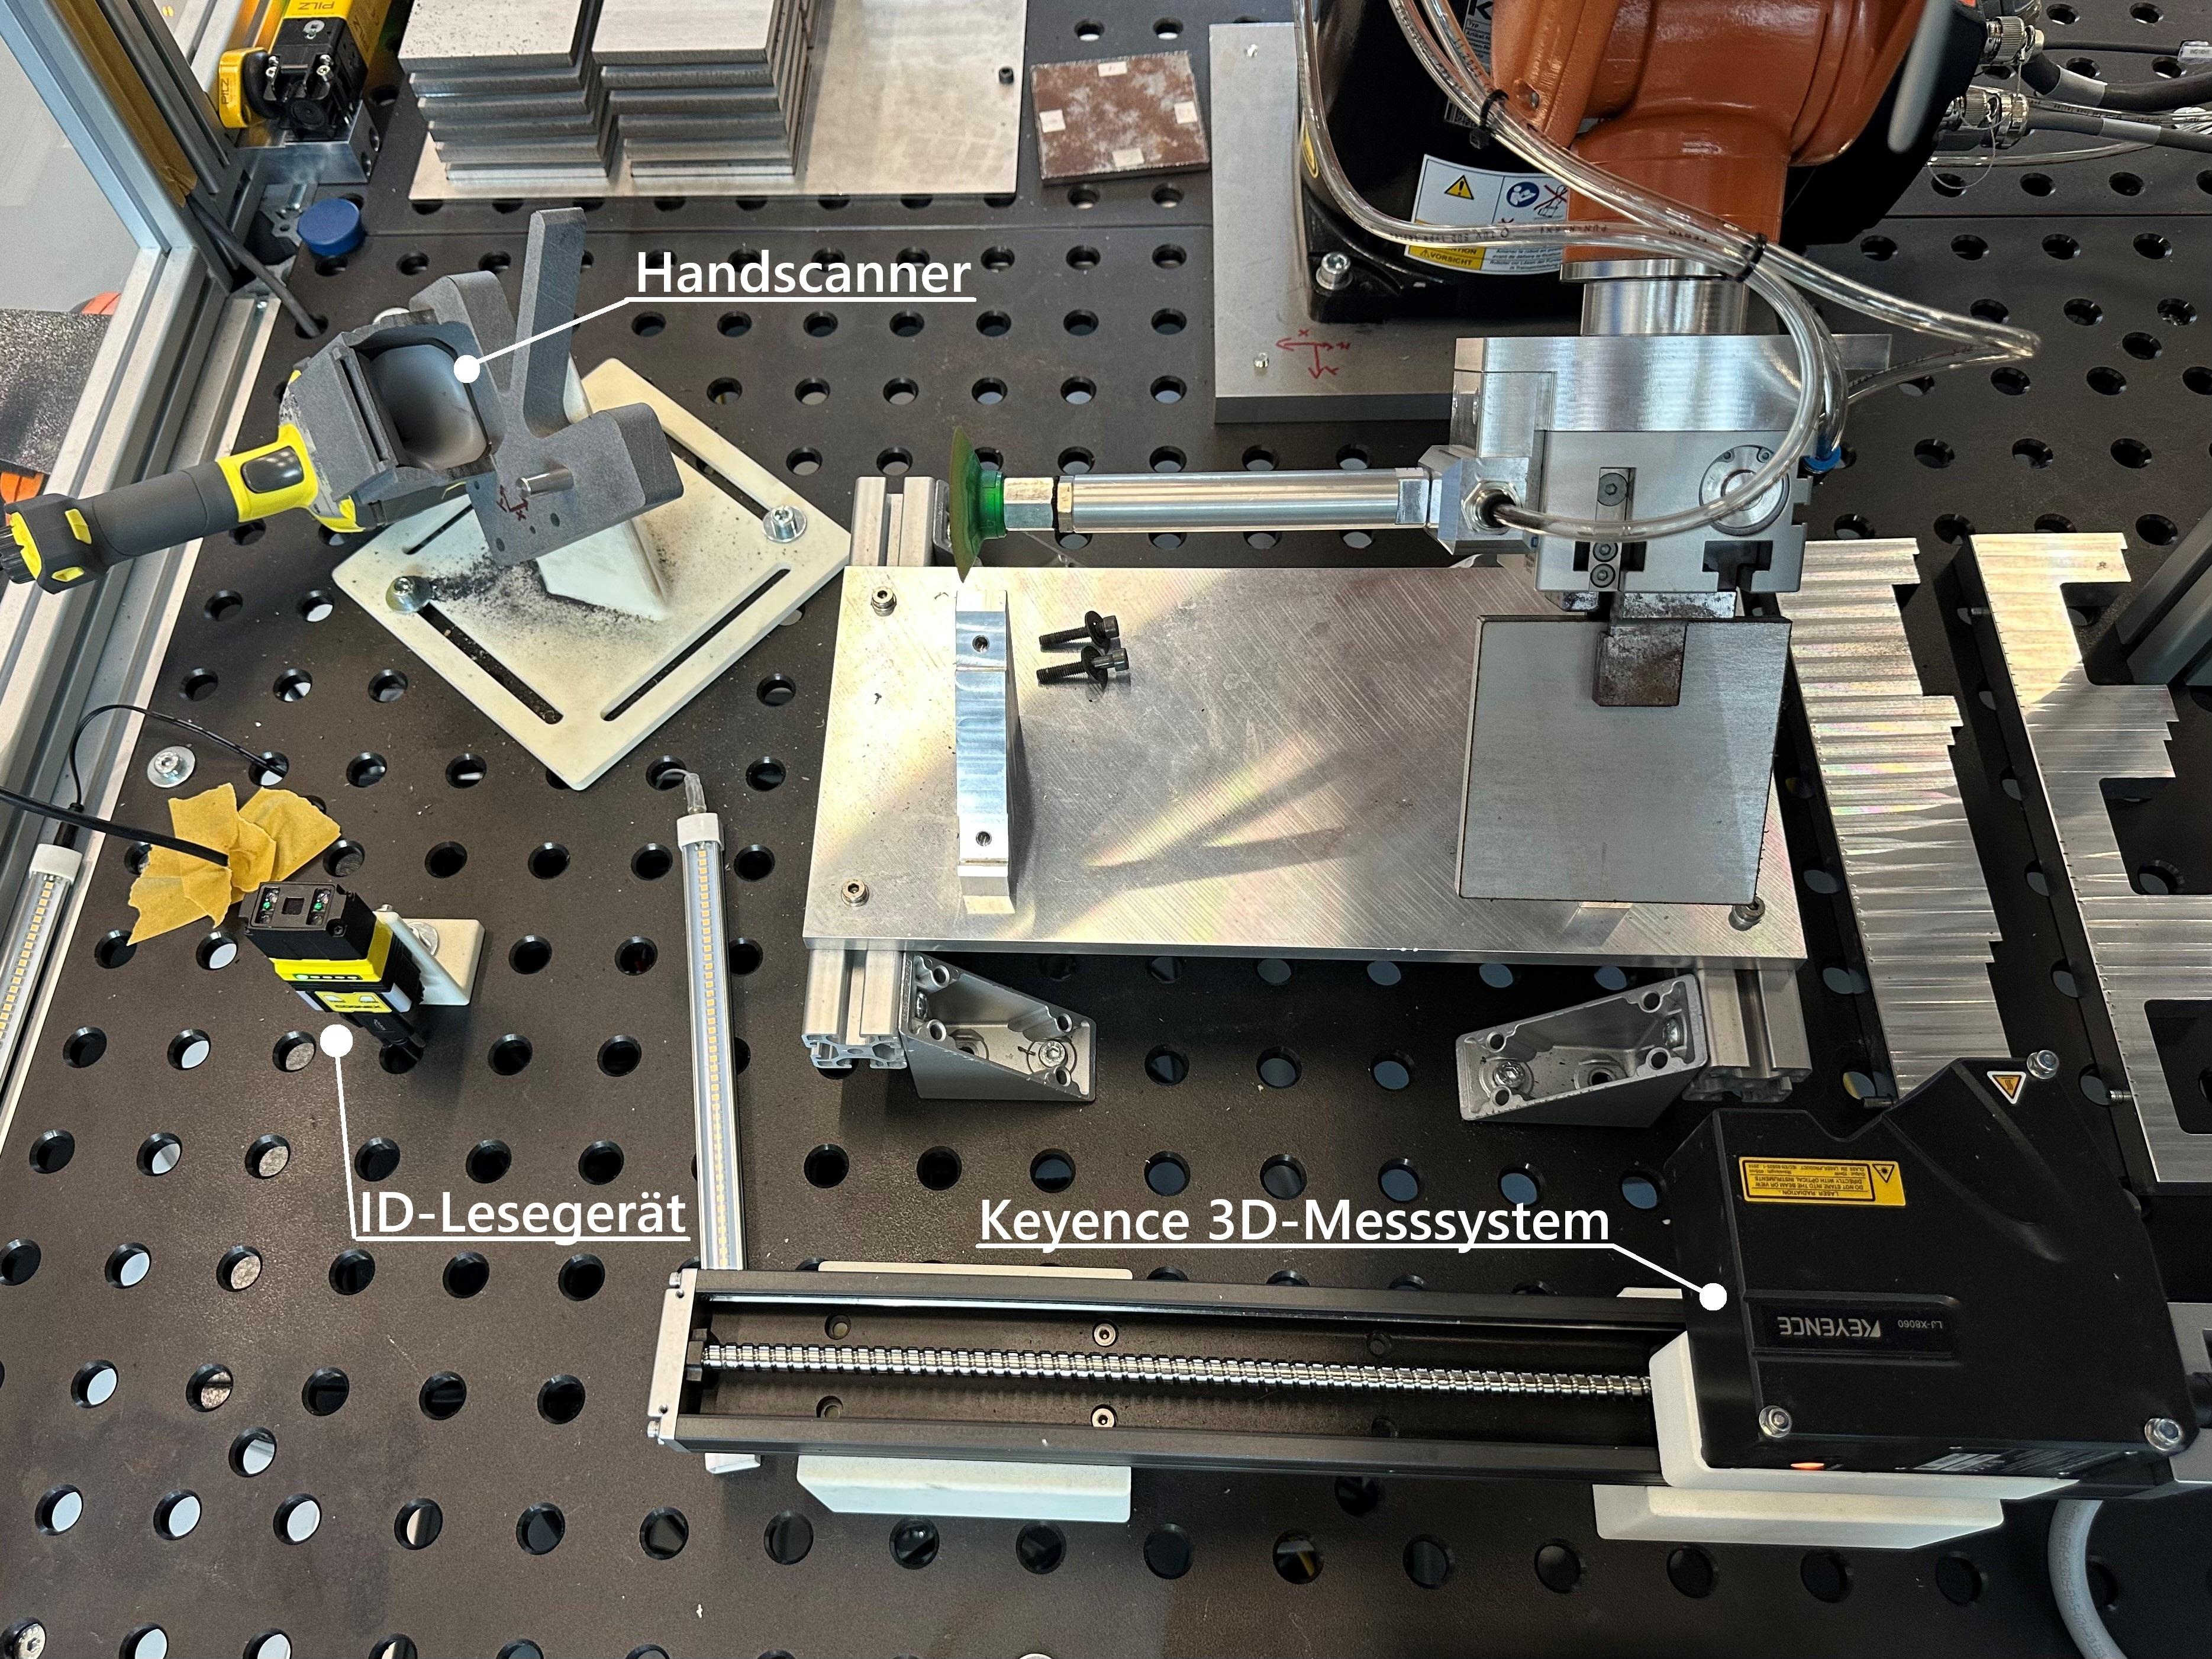
\includegraphics[width=0.6\linewidth]{handscanner_keyence.jpg}
    \caption{Handscanner (1), ID-Lesegerät (2), Keyence 3D-Messsystem (3) in der Messzelle}
    \label{fig:handscanner_barcodelesegerät_keyence}
\end{figure}

\newpage

Zur vollständigen Dokumentation werden die Schnittkanten zudem mit einer Industriekamera und einem stationären Smartphone-Setup unter verschiedenen Beleuchtungsbedingungen aufgenommen. Die Kombination aus unterschiedlichen Kameras und Beleuchtungen erhöht die Robustheit der visuellen Beurteilbarkeit und unterstützt die spätere manuelle Nachvollziehbarkeit von Auffälligkeiten. Die erfassten Messdaten des Werkstücks, sowie die daraus abgeleiteten Kenngrößen der Proben-ID zugeordnet und in die zentrale Datenbank überführt.

Die Abbildung~\ref{fig:smartphone_industriekamera} zeigt die zuvor beschriebenen Komponenten der Messzelle. Oben im Bild ist das Smartphone (4) mit LED-Ringlicht zu sehen, welches die Schnittkante aus einem flachen Winkel aufnimmt. Unten im Bild ist die Industriekamera (5) mit Auflichtbeleuchtung dargestellt, welche die Schnittkante ebenfalls aus einem flachen Winkel erfasst. Beide Kameras sind fest in der Messzelle montiert und werden automatisch durch den Roboter angesteuert.
\begin{figure}[htbp]
    \centering
    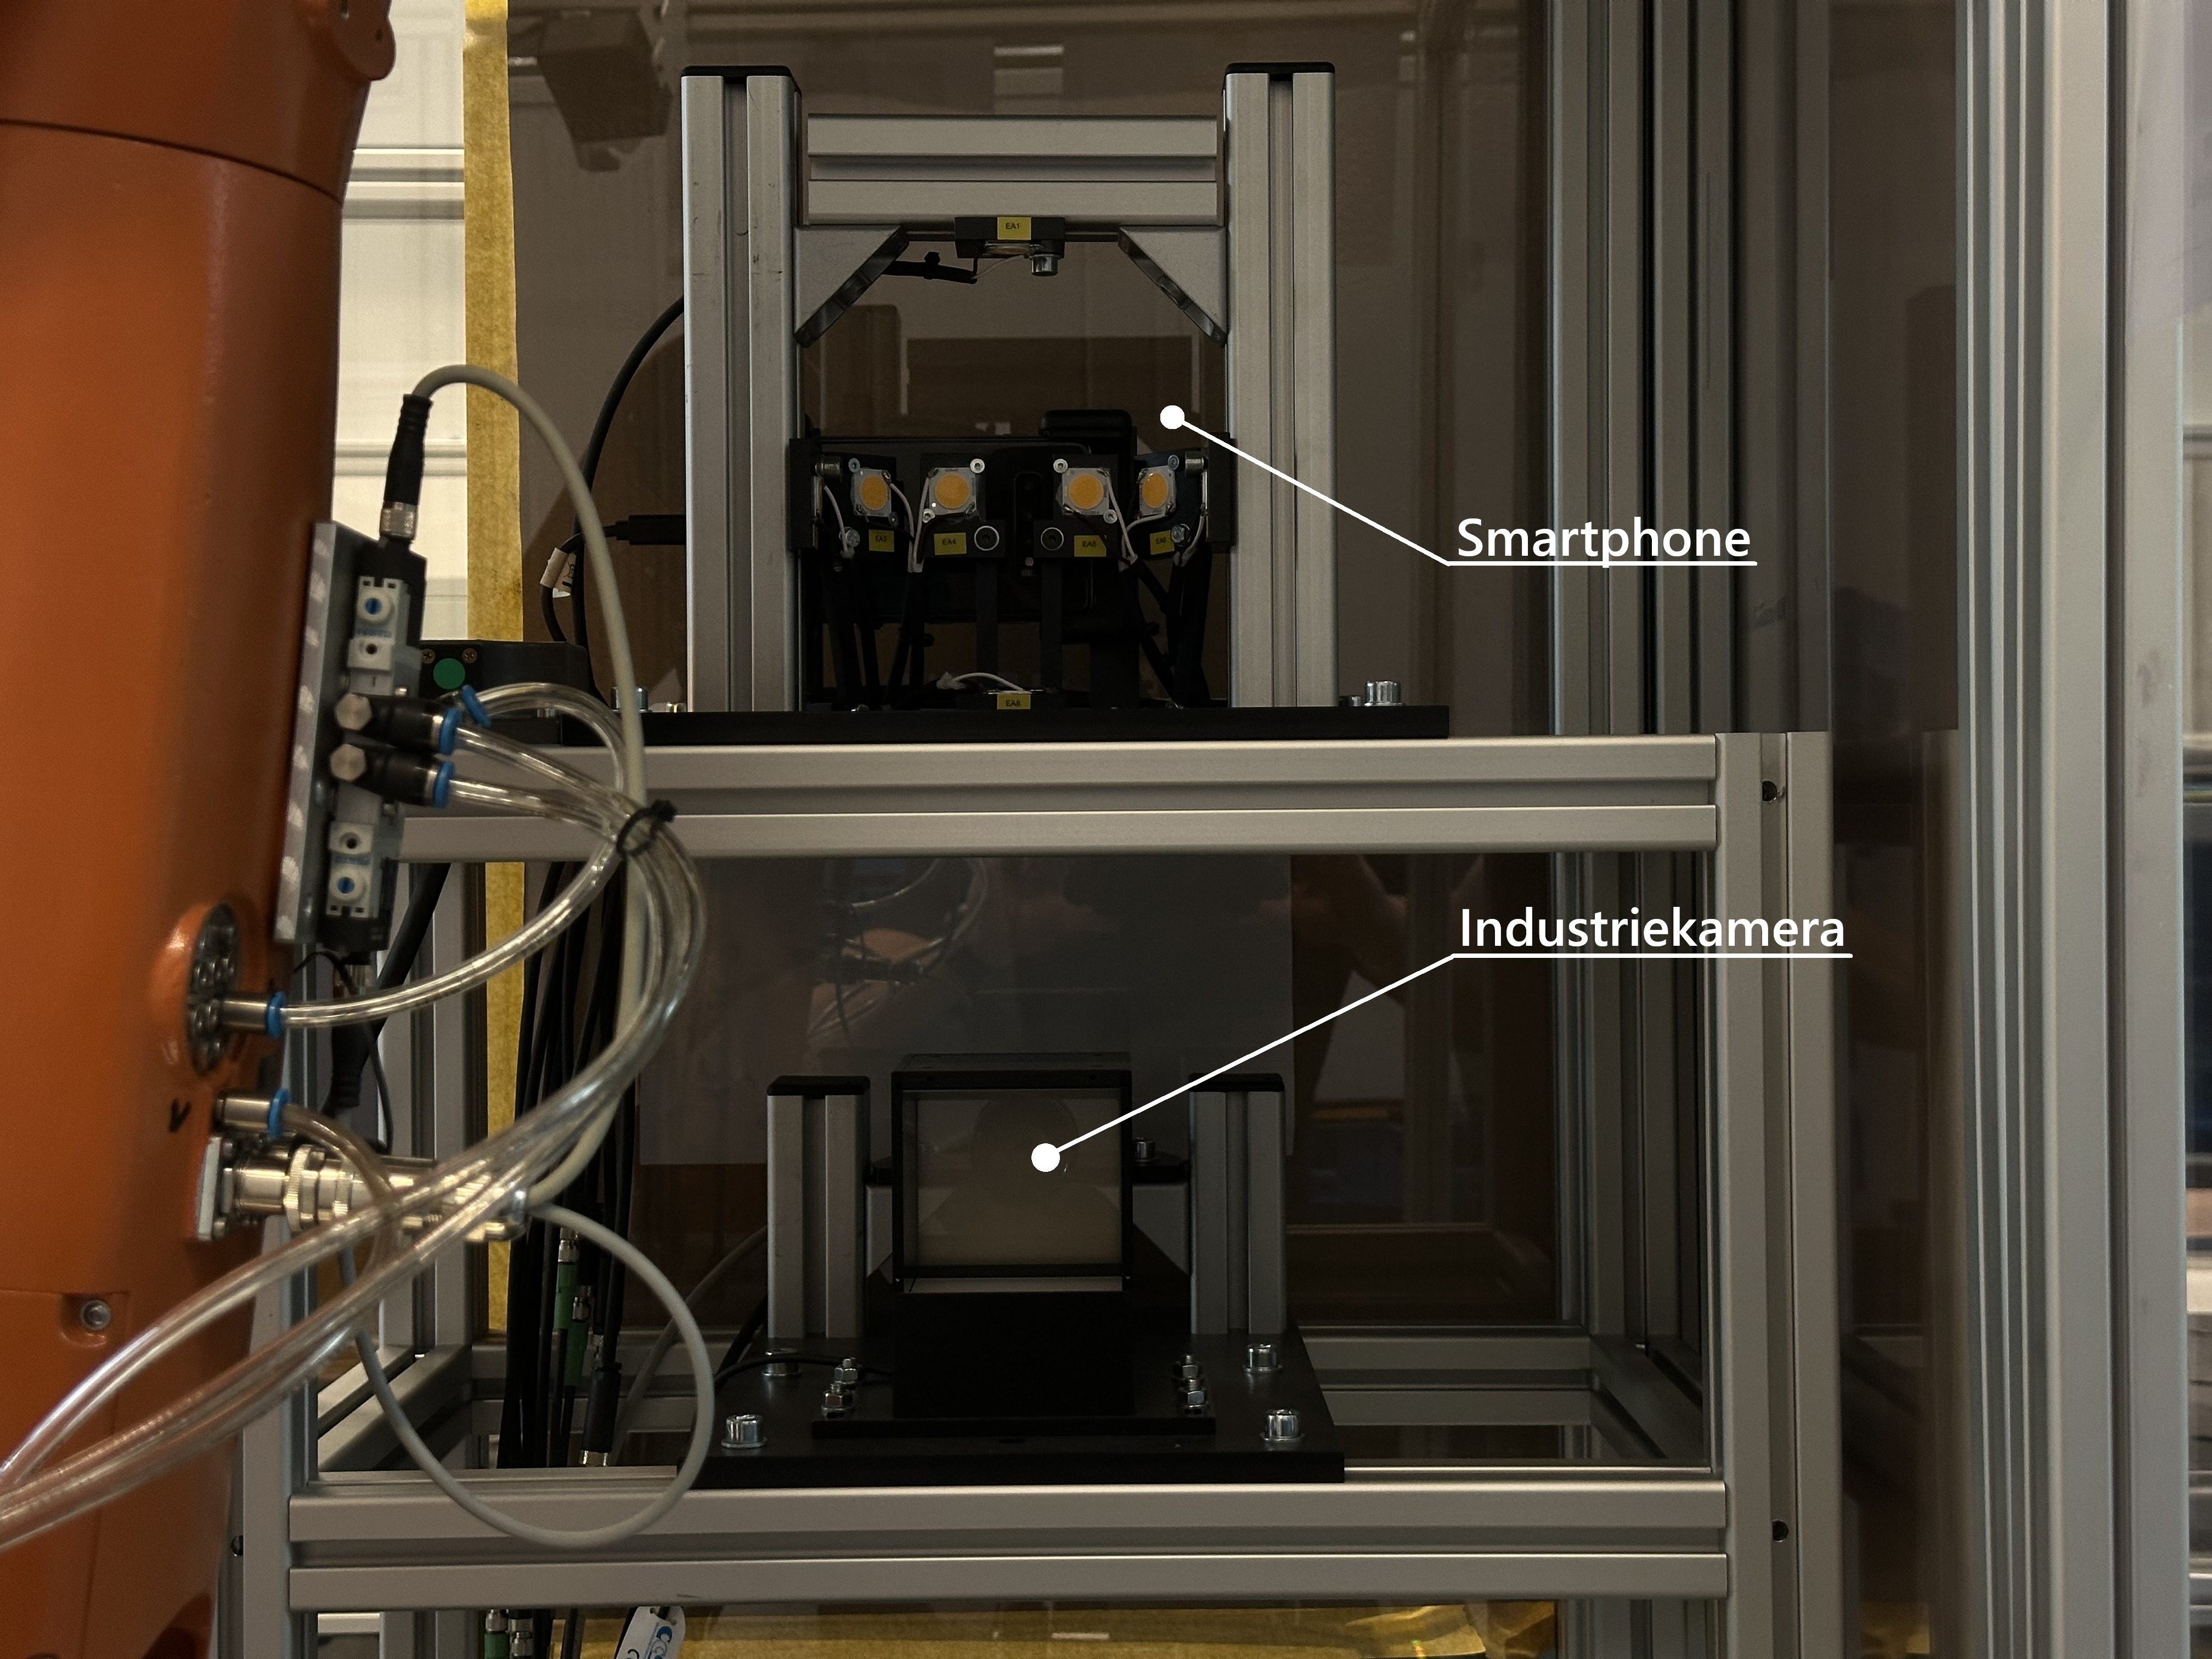
\includegraphics[width=0.6\linewidth]{smartphone_industriekamera.jpg}
    \caption{Smartphone (4) und Industriekamera (5) in der Messzelle}
    \label{fig:smartphone_industriekamera}
\end{figure}

Nach der Datenerfassung werden aus der 3D-Messung die tatsächlichen Kenngrößen der Schnittkante berechnet und den Ergebnissen der bildbasierten Qualitätsschätzung gegenübergestellt. Dieser Abgleich ermöglicht die Beurteilung der Übereinstimmung zwischen qualitativer, bildgestützter Bewertung und quantitativer Geometriemessung. Die beschriebenen Messschritte werden für alle vier Schnittkanten jedes Bauteils identisch wiederholt. Abschließend legt der Roboter die vollständig vermessenen Proben an der Endstation geordnet ab.

Anbei ist ein besipielhafter Vergleich der geschätzten Kenngrößen einer Schnittkante im Vergleich zu den gemessenen Kenngrößen in den Abbildungen  ~\ref{fig:burr_true_pred} und ~\ref{fig:roughness_true_pred} dargestellt. Es sind jeweils zwei Diagramme zu sehen, einer für den Gratwert und einer für die Rauheit. Auf den y-Achsen sind die geschätzten Kenngrößen und auf der x-Achse die gemessenen Kenngrößen aufgetragen. Idealerweise liegen alle Punkte auf der Diagonalen, was eine perfekte Übereinstimmung zwischen Schätzung und Messung bedeuten würde. In disem Beispiel Überschätzt das KI-Modell den Rauheitswert leicht, whärend der Gratwert überwiegend "gut" geschätzt wird. Mit einer leichten Abweichung ist stets zu rechnen, da die bildbasierte Schätzung eine Näherung darstellt und nicht alle Details der 3D-Messung erfassen kann.

\begin{figure}[h!]
    \centering
    \begin{minipage}{0.48\textwidth}
        \centering
        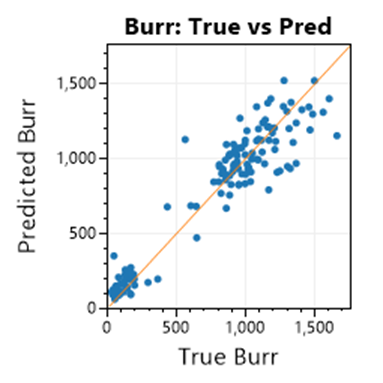
\includegraphics[width=\linewidth]{qualitatsschatzung_burr.png}
        \caption{Vergleich zwischen vorhergesagten und tatsächlichen Werten für den Grat (Burr).}
        \label{fig:burr_true_pred}
    \end{minipage}
    \hfill
    \begin{minipage}{0.48\textwidth}
        \centering
        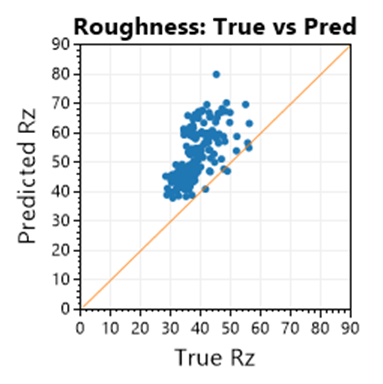
\includegraphics[width=\linewidth]{qualitatsschatzung_roughness.png}
        \caption{Vergleich zwischen vorhergesagten und tatsächlichen Werten für die Rauheit (Roughness).}
        \label{fig:roughness_true_pred}
    \end{minipage}
\end{figure}



\newpage

\section{Anpassung des Handscanner-Setups}
\label{chap:handscanner-setup}

Für die bildgestützte Qualitätsschätzung werden die mit dem Handscanner aufgenommenen Schnittkantenbilder als zentrale Eingangsgröße verwendet. Die bisher im Einsatz befindlichen Aufnahmeparameter waren für Baustahl optimiert. Baustahl weist im Vergleich zu Edelstahl eine geringere Oberflächenreflexion und eine tendenziell matte Erscheinung auf. Werden diese Einstellungen unverändert auf Edelstahl angewandt, führt die höhere Reflexion zu Bildartefakten und zu einer unzureichenden Abbildung der relevanten Mikrostruktur \parencite{ZahnerStainlessReflect}. In der Folge würden Grate (\emph{engl. Burr}) unterrepräsentiert und die Rauheit (\emph{engl. Roughness}) potenziell verfälscht erscheinen. Da die Klassifikation der Bildqualität und die darauf basierende Schätzung von \emph{Burr} und \emph{Roughness} unmittelbar in die Parametrierung des Laserschneidprozesses zurückwirken, ist eine werkstoffabhängige Anpassung des Handscanner-Setups zwingend erforderlich.

Das Aufnahmeprotokoll sieht pro Schnittkante drei Bilder vor: (i) ein bewusst dunkler belichtetes Bild, das primär der Beurteilung der Schnittflächenrauheit dient, sowie (ii) zwei überbelichtete Bilder, die gemeinsam mit dem ersten zu einem HDR-Komposit zusammengeführt werden, um die Kontur und Ausprägung des Grats sicher zu erfassen. Die Kalibrierung der Belichtung erfolgt schrittweise. Zunächst wird die Belichtungszeit für das Rauheitsbild so eingestellt, dass die Textur der Schnittfläche ohne Sättigung und mit klarer Detailzeichnung sichtbar ist. Diese Entscheidung erfolgt in dieser Phase bewusst subjektiv, jedoch anhand vorab definierter visueller Kriterien, wie z.B. ausreichender Tonwertumfang und erkennbarer Strukturkontrast. Im Anschluss werden die Belichtungsparameter der beiden HDR-Bilder iterativ variiert, bis der Grat entlang der Schnittkante über den gesamten Bildbereich eindeutig detektierbar ist, ohne dass umliegende Bereiche vollständig verloren gehen. Da die HDR-Komposition durch die Eingangsbilder beeinflusst wird, erfolgt die Abstimmung der HDR-Belichtungen stets nach der Festlegung des Rauheitsbildes. 
Die Abbildungen~\ref{fig:burr_baustahl},~\ref{fig:burr_edelstahl}, ~\ref{fig:roughness_baustahl} und ~\ref{fig:roughness_edelstahl} zeigen exemplarisch die finalen Handscanner Bilder, welche für die Qualitätsschätzung genutzt werden, für Edelstahl im Vergleich zu den bisherigen Bildern für die Qualitätsschätzung von Baustahl. In den Abbildungen ist jeweils die gleiche Schnittkante eines Blechteils aus den geschnittenen Experimentalplänen dargestellt mit einer Dicke von 15 mm.

\begin{figure}[htbp]
  \centering
  \begin{minipage}{0.48\linewidth}
    \centering
    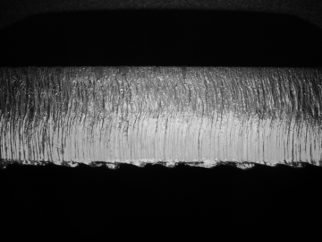
\includegraphics[width=\linewidth]{burr_baustahl.png}
    \caption{Handcanner Bild für die Gratschätzung (Baustahl)}
    \label{fig:burr_baustahl}
  \end{minipage}\hfill
  \begin{minipage}{0.48\linewidth}
    \centering
    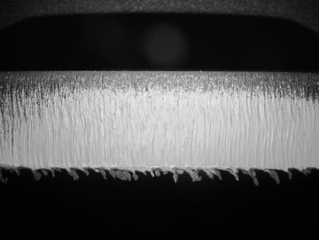
\includegraphics[width=\linewidth]{burr_edelstahl.png}
    \caption{Handcanner Bild für die Gratschätzung (Edelstahl)}
    \label{fig:burr_edelstahl}
  \end{minipage}
\end{figure}

\begin{figure}[htbp]
  \centering
  \begin{minipage}{0.48\linewidth}
    \centering
    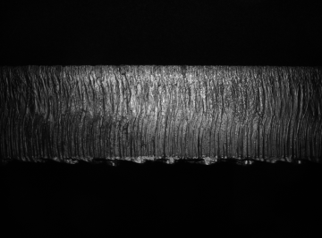
\includegraphics[width=\linewidth]{roughness_baustahl.png}
    \caption{Handscnanner Bild für die Rauheitsschätzung (Baustahl)}
    \label{fig:roughness_baustahl}
  \end{minipage}\hfill
  \begin{minipage}{0.48\linewidth}
    \centering
    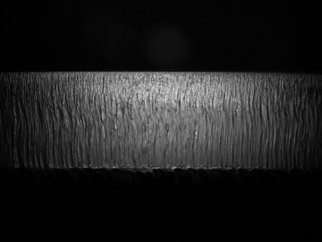
\includegraphics[width=\linewidth]{roughness_edelstahl.png}
    \caption{Handscanner Bild für die Rauheitsschätzung (Edelstahl)}
    \label{fig:roughness_edelstahl}
  \end{minipage}
\end{figure}

Zur Sicherstellung der Kompatibilität mit dem bestehenden KI-Modell wird die Anpassung an Referenzaufnahmen aus der bereits validierten Baustahlkonfiguration ausgerichtet. Praktisch bedeutet dies, dass eine Baustahlschnittkante mit den etablierten Baustahleinstellungen aufgenommen wird und die Edelstahlaufnahmen so justiert werden, dass die resultierenden Bildcharakteristika in qualitativer Hinsicht vergleichbar sind. Auf diese Weise wird gewährleistet, dass die Edelstahlbilder in das bestehende Modell eingebunden und mit den vorhandenen Trainings- und Bewertungsroutinen verarbeitet werden können.

Zur konsistenten Anwendung der angepassten Handscanner-Parameter wird das Messzellen-Skript so erweitert, dass das passende Setup automatisiert auf Basis der Bauteilbezeichnung gewählt wird. Die Benennung folgt dem Schema
\texttt{Maschinenname-\allowbreak Experimentalplanname-\allowbreak Materia
lnummer-\allowbreak Bauteildicke-\allowbreak Bauteilnummer},
z.\,B.\ \texttt{A02280E0005-\allowbreak AiMuWrCjd0-\allowbreak 3-\allowbreak 050-\allowbreak 0176}.
Die folgende Abbildung ~\ref{fig:probenID} zeigt eine Beispiel-Proben-ID eines Blechstücks aus den Experimentalplänen mit den einzelnen Segmenten.

\begin{figure}[htbp]
    \centering
    \includegraphics[width=0.7\linewidth]{Werkstück_Proben-ID.jpg}
    \caption{Beispiel-Proben-ID eines Blechstücks aus den Experimentalplänen}
    \label{fig:probenID}
\end{figure}

Das Skript parst die Zeichenkette, prüft die Zahl nach dem zweiten Bindestrich und lädt abhängig davon die vordefinierten Handscanner-Einstellungen für den jeweiligen Werkstoff. Auf diese Weise wird sichergestellt, dass die für Edelstahl kalibrierten Belichtungen und Aufnahmeparameter reproduzierbar zur Anwendung kommen und die so erzeugten Bilder ohne systematische Verzerrungen in die Qualitätsmodellierung eingehen. Dies ist im folgendem C-Sharp Quellcode ~\ref{lst:messzellen-routing} dargestellt und im Messzellenskript inplementiert.

\begin{lstlisting}[language={[Sharp]C}, caption={Werkstoffabhängiges Routing der Handscanner-Setups}, label={lst:messzellen-routing}]
public static string NameParserMaterial(string input)
{
    if (string.IsNullOrWhiteSpace(input))
        return "ST";                                // Fallback-Wert

    // Position des ersten und zweiten Bindestrichs ermitteln
    int firstDash = input.IndexOf('-');
    int secondDash = firstDash >= 0
                   ? input.IndexOf('-', firstDash + 1)
                   : -1;

    // Prüfen, ob ein zweiter Bindestrich und ein Zeichen dahinter existieren
    if (secondDash < 0 || secondDash + 1 >= input.Length)
        return "ST";                                // Fallback-Wert

    char digit = input[secondDash + 1];             // Ziffer einlesen

    // Zuordnung: 1 → "ST", 2 → "ST", 3 → "SS" (bei Bedarf anpassen)
    return digit switch
    {
        '1' => "ST",
        '2' => "ST",
        '3' => "SS",
        _ => "ST"                                   // Default
    };
}
\end{lstlisting}

\section{Optimierung der Vektorberechnung aus 3D-Punktwolken}

Die mit dem Keyence-System aufgenommene 3D-Punktwolke der Schnittkante bildet die Grundlage für die geometrische Qualitätsauswertung. In der bestehenden Auswertepipeline wird die Punktwolke zunächst segmentiert und in ein lokales Kantenkoordinatensystem überführt. Anschließend erfolgt eine Projektion aus der dreidimensionalen Repräsentation in einen zweidimensionalen Profilverlauf, sodass ein 2D-Vektor entsteht, der den Verlauf des Schneidgrats entlang der Schnittkante beschreibt. Diese Vorgehensweise wurde ursprünglich für Baustahl entwickelt und auf dessen charakteristisch eher wellige, kontinuierliche Gratmorphologie abgestimmt.

Die nachfolgend beschriebenen Anpassungen betreffen ausschließlich den \textbf{Grat-/Burr}-Kanal unterteilt in der Ausreißererkennung von Messdaten und der darauffolgenden Interpolation. Für die Rauheitsanalyse werden die in der Baustahl-Pipeline etablierten Einstellungen übernommen. Aus interner Erfahrung zeigt die Rauheitsprüfung eine stabile und konsistente Bewertung.

Bei Edelstahl zeigt sich eine abweichende, ausgeprägt zackige Gratstruktur mit höheren lokalen Gradienten und diskontinuierlichen Profilabschnitten. Die bislang implementierte Outlier-Korrektur ist konzipiert zur Eliminierung sporadischer Messfehler bei Baustahl. Demnach stuft diese den Gratverlauf von Edelstahl fälschlich als Ausreißer ein und glättet sie übermäßig. Dadurch werden relevante Merkmale des Edelstahlgrats unterdrückt und der resultierende Vektorverlauf in Richtung eines künstlich „glatten“ Profils verzerrt.

Erschwerend kommt hinzu, dass im Messprozess partiell überbeschattete Bereiche auftreten können, die vom Sensor nicht erfasst werden. In der bisherigen Pipeline werden solche Lücken durch Interpolation geschlossen, deren Parameter auf die kontinuierlichen Profile von Baustahl zugeschnitten sind. Für den zackigen Edelstahlgrat führt dies zu einer zu starken Annäherung an glatte Zwischenverläufe und damit zu einem Verlust an formcharakteristischer Information.

Zur materialspezifischen Anpassung werden daher zwei Kernmodule überarbeitet. Die Ausreißererkennung \cref{sec:Outlier Detection/Correction} mit nachgelagerter Korrektur und die Interpolation \cref{sec:Interpolation} fehlender Stützstellen. In der Ausreißererkennung werden die Schwellwerte und die zugrunde liegenden Sensitivitätsmaße an die höhere lokale Krümmung und den gesteigerten Kantenkontrast des Edelstahlgrats angepasst. Ziel ist eine Differenzierung zwischen echten Messfehlern und materialtypischen Hochfrequenzanteilen. Entsprechend werden Glättungsschritte zurückgenommen, sodass signifikante Gratflanken erhalten bleiben. 

Für die Interpolation wird ein konservativer Ansatz gewählt, der Lückenschlüsse bevorzugt entlang lokal konsistenter Nachbarschaften vornimmt und globale, stark glättende Approximationen vermeidet. Damit wird erreicht, dass der rekonstruierte 2D-Vektor fehlende Messpunkte plausibel ergänzt, ohne die charakteristische Zackigkeit des Edelstahlgrats zu nivellieren.

\subsection{Outlier Detection/Correction des Gratverlaufs}
\label{sec:Outlier Detection/Correction}

Die Ausreißerbehandlung im \textbf{Burr}-Kanal erfolgt zweistufig. Zunächst werden potenzielle Ausreißerpunkte durch den Vergleich des gemessenen Profils mit einem lokal geglätteten Referenzsignal identifiziert. Anschließend werden die dadurch entstehenden Lücken kontrolliert und rekonstruiert. In \texttt{outlier\_correction\_burr} wird das Höhenprofil \texttt{z\_vec} mittels gleitendem Mittelwert (\texttt{np.convolve} mit der Fensterlänge \texttt{window}) geglättet. Die absolute Abweichung \(\Delta=\lvert z-\overline{z}_{\text{MA}}\rvert\) wird punktweise gegen den Schwellwert \texttt{threshold} geprüft. Punkte oberhalb des Schwellwertes bilden die Ausreißermaske. Ist der Anteil markierter Punkte größer als \texttt{max\_nan\_values\_perc}, wird der Vorgang verworfen (\texttt{None}). Andernfalls werden die Ausreißer zu \texttt{NaN} gesetzt und mit \texttt{smooth\_nan\_values} rekonstruiert, um numerisches Rauschen zu reduzieren, ohne relevante Strukturen zu nivellieren.

Die Funktion \texttt{outlier\_correction\_profile\_lines} setzt denselben Ansatz für einzelne Profilzeilen um, verwendet jedoch standardmäßig einen robusten gleitenden Median (\texttt{median=True}) als Referenzsignal. Aus der Abweichung zum Referenzsignal wird eine Ausreißermaske gebildet und über \texttt{max\_outlier\_values\_perc} validiert. Markierte Punkte werden zu \texttt{NaN} gesetzt und anschließend nur dann interpoliert, wenn die Lückenlänge die Vorgabe \texttt{max\_gap} nicht überschreitet (\texttt{interpolate\_limited\_nans}).Die Rauheitsanalyse nutzt unverändert die etablierten Baustahl-Einstellungen, hierfür erfolgt keine Umparametrisierung.

\begin{lstlisting}[language=Python, caption={Outlier Detection/Correction in der Profilvorverarbeitung (Burr-Kanal)}, label={lst:outlier-correction}]
def outlier_correction_burr(x_vec, z_vec, threshold=0.04, window=20, max_nan_values_perc=0.4):
    """
    Entfernt Ausreißer anhand eines Moving-Average-Vergleichs.
    """
    z_vec = np.copy(z_vec)
    z_smoothed = np.convolve(z_vec, np.ones(window) / window, mode='same')
    difference = np.abs(z_vec - z_smoothed)

    outlier_mask = difference > threshold
    num_outliers = np.sum(outlier_mask)

    if num_outliers / len(z_vec) > max_nan_values_perc:
        return None, None

    z_vec[outlier_mask] = np.nan
    z_vec_clean = smooth_nan_values(x_vec, z_vec)

    return x_vec, z_vec_clean


def outlier_correction_profile_lines(line, outlier_threshold=0.04, window_size=30,
                                     median=True, max_outlier_values_perc=0.35, max_gap=5):
    """
    Entfernt Ausreißer in Höhenprofilen basierend auf Median- oder Mittelwert-Vergleich.
    """
    Z_series = pd.Series(line)
    tmp_line = line.copy()

    if median:
        moving_avg = Z_series.rolling(window_size, min_periods=5, center=True).median()
    else:
        moving_avg = Z_series.rolling(window_size, min_periods=5, center=True).mean()

    difference = np.abs(line - moving_avg)
    id_outlier = difference > outlier_threshold
    count_outlier = np.sum(id_outlier)

    if count_outlier / len(line) > max_outlier_values_perc:
        return None, None

    tmp_line[id_outlier] = np.nan
    tmp_line = interpolate_limited_nans(tmp_line, max_gap=max_gap)

    return tmp_line, moving_avg
\end{lstlisting}

In der Edelstahl-Pipeline wurden die Schwellwerte der Burr-Outlier-Korrektur angehoben und das Fenster leicht verkürzt, um zackige, materialspezifische Hochfrequenzanteile nicht fälschlich als Ausreißer zu markieren. Zum Vergleich sind nachfolgend die verwendeten Parameter für Edelstahl sowie die bisherige Baustahl-Konfiguration aufgeführt (siehe auch Quellcode~\ref{lst:params-outlier-stainless} und Quellcode~\ref{lst:params-outlier-mild}). Für die Rauheitsanalyse wurden keine Parameteränderungen vorgenommen.

\begin{lstlisting}[caption={Pipeline-Parameter Outlier Correction (Edelstahl, Burr-Kanal)}, label={lst:params-outlier-stainless}]
# Parameter burr outlier correction (Edelstahl)
burr_outlier_threshold : 0.06  # Threshold for Moving Average Difference Filter [mm]
burr_outlier_window    : 9     # Window for Moving Average Difference Filter [samples]
\end{lstlisting}

\begin{lstlisting}[caption={Pipeline-Parameter Outlier Correction (Baustahl, Burr-Kanal)}, label={lst:params-outlier-mild}]
# Parameter burr outlier correction (Baustahl)
burr_outlier_threshold : 0.03  # Threshold for Moving Average Difference Filter [mm]
burr_outlier_window    : 10    # Window for Moving Average Difference Filter [samples]
\end{lstlisting}

\subsection{Interpolation des Gratverlaufs}
\label{sec:Interpolation}

Die Interpolation rekonstruiert fehlende Messwerte (\texttt{NaN}), die durch Ausreißerkennzeichnung oder unvollständige Erfassung entstehen. Ziel ist die Wiederherstellung eines plausiblen Gratverlaufs, daher werden nur kurze, lokal begrenzte Lücken gefüllt und größere Ausfälle bleiben markiert. Durch die angepasste Ausreißererkennung werden weniger echte Messpunkte fälschlich als Ausreißer markiert, sodass deutlich weniger Lücken entstehen und nicht mehr unnötig interpoliert wird. Am Interpolationsskript wurden keine Änderungen vorgenommen. Alle Konstanten bleiben unverändert, insbesondere die maximale Lückenlänge sowie Glättungs- und Fensterparameter. Der zugehörige Quellcode ist im Anhang dokumentiert.
Die Validierung desssen erfolgt im folgendem Kapitel ~\ref{sec:validierung-burr}.

\section {Validierung der Messoptimierungen}
\label{sec:validierung-burr}

Im folgendem Kapitel werden die verbesserten Messmethoden für die Grat- und Rauheitsanalyse validiert, um bestenfalls die Optimierung für Datenerfassung zu nutzen, so dass das KI-Modell neu trainiert werden kann. 

\subsection{Validierung der verbesserten Ausreißererkennung im Burr-Kanal}

In diesem Abschnitt werden die edelstahl-optimierten Einstellungen der Ausreißererkennung validiert. Verglichen wird die frühere Baustahl-Parametrierung mit der angepassten Erkennung für Edelstahl.

Die Abbildung~\ref{fig:burr-compare} den Vergleich der verbsserten und der unverbeserten Ausreißererkennung. Hierfür wurden jeweils das gleiche Sektioonsbild des gleichen Edelstahlblechs. Die rote Linie ist der abgeleitete Burr-Vektor. Auf dem linken Schaubild ist die unverbesserte Ausreißererkennung erkennbar, welche für Baustahl werdet wird und rechts die verbesserte Ausreißererkennung. Demnach ist der verbesserte Verlauf durchgängig, es entstehen weniger fehlerhafte Lücken und die interpolierten Abschnitte sind plausibler. Quantitativ sinkt der Burr-Wert der gezeigten Sektion von \(681{,}99\,\mu\mathrm{m}\) (Baustahl-Parameter) auf \(650{,}88\,\mu\mathrm{m}\) (Edelstahl-Parameter), jedoch erfolgt die einschätzende Bewertung visuell. Es wird geprüft, wie gut die rote Linie dem sichtbaren Gratverlauf folgt.  
\begin{figure}[htbp]
  \centering
  \begin{minipage}[t]{0.48\linewidth}
    \centering
    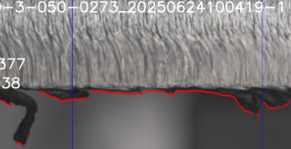
\includegraphics[width=\linewidth]{outlier_detection_baustahl.png}
    \vspace{0.3em}
    {\small\emph{Unverbesserte Ausreißererkennung: sichtbare Lücken und Fehlverfolgungen.}}
  \end{minipage}\hfill
  \begin{minipage}[t]{0.48\linewidth}
    \centering
    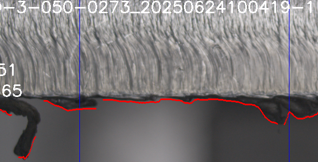
\includegraphics[width=\linewidth]{outlier_detection_edelstahl.png}
    \vspace{0.3em}
    {\small\emph{Verbesserte Ausreißererkennung: durchgängiger Verlauf, plausiblere Interpolation.}}
  \end{minipage}
  \caption[Ausreißererkennung im Burr-Kanal]{Links ist die unverbesserte Ausreißererkennung erkennbar, welche für Baustahl werdet wird und rechts die verbesserte Ausreißererkennung. Die rote Kurve ist der abgeleitete Burr-Vektor.}
  \label{fig:burr-compare}
\end{figure}

Demnach ist die verbesserte Ausreißererkennung für Edelstahl validiert. Die Rauheitsanalyse wurde nicht verändert, da diese in internen Erfahrungen eine stabile und konsistente Bewertung zeigt.

\subsection{Validierung der bestehenden Rauheitsanalyse an den neuen Edelsdtahldaten}
In diesem Abschnitt wird die Rauheitsanalyse validiert. Die Berechnungsmethode bleibt unverändert. Die Belichtung des Handscanners wurde so angepasst, dass die Struktur der Schnittfläche zuverlässig erfasst wird (siehe Abschnitt~\ref{chap:handscanner-setup}). Zur Prüfung der Eignung wurde die bestehende Rauheitsberechnung auf die neuen Bilder von Edelstahlblechen angewendet und auf mögliche Ausreißer in den resultierenden Rauheitswerten untersucht. Es traten keine systematischen Ausreißer auf, daher wird die Berechnung vorerst unverändert weitergeführt. Anpassungen werden erst nach weiterführenden Modelltrainings geprüft.


% \blinddocument
%%% Ende des eigentlichen Inhalts %%%


%%% Quellenverzeichnisse (keine Anpassung nötig) %%%
\clearpage
\literaturverzeichnis
\startAnhang

\listofanhang
\clearpage

\anhang{So funktioniert's}

\lstset{language=TeX, % hervorzuhebende Keywords definieren
  morekeywords={anhang, anhangteil}
}


Um den Anforderungen der Zitierrichtlinien nachzukommen, wird das Paket \verb|tocloft| verwendet. Jeder Anhang wird mit dem (neu definierten) Befehl \lstinline|\anhang{Bezeichnung}| begonnen, der insbesondere dafür sorgt, dass ein Eintrag im Anhangsverzeichnis erzeugt wird. Manchmal ist es wünschenswert, auch einen Anhang noch weiter zu unterteilen. Hierfür wurde der Befehl \lstinline|\anhangteil{Bezeichnung}| definiert.

In~\ref{anhang:abbildung} finden Sie eine bekannte Abbildung und etwas Source Code in~\ref{anhang:sourcecode}. 

\anhangteil{Wieder mal eine Abbildung}\label{anhang:abbildung}
\begin{figure}[htb]
\centering
\includegraphics[width=0.9\linewidth]{graphics/dhbw.png}
\caption{Mal wieder das DHBW-Logo.}
\end{figure}

\anhangteil{Etwas Source Code}\label{anhang:sourcecode}
\lstinputlisting{includes/HelloWorld.java}


%%% Ende Quellenverzeichnisse %%%


%%% Erklärung (keine Anpassungen nötig) %%%
% steht ganz am Ende des Dokuments
\cleardoublepage
%\clearpage

\thispagestyle{empty}
\DEoEN{%
{\LARGE\textsf{\textbf{Erklärung zur Verwendung generativer KI-Systeme}}\bigskip}

Bei der Erstellung der eingereichten Arbeit habe ich auf künstlicher Intelligenz (KI) basierte Systeme benutzt: 

\begin{enumerate}
\item[$\boxtimes$] ja
\item[$\square$] nein\footnote{%
Die Erklärung ist in jedem Fall zu unterzeichnen, auch wenn Sie keine KI-Systeme genutzt haben und Ihr Kreuz bei \enquote{nein} gesetzt haben.}
\end{enumerate}

% Falls nein: Rest des Blocks entfernen, Unterschrift aber beibehalten

Falls ja: Die nachfolgend aufgeführten auf künstlicher Intelligenz (KI) basierten Systeme habe ich bei der Erstellung der eingereichten Arbeit benutzt:

\begin{enumerate}
\item
\item
\item \ldots
\end{enumerate}

Ich erkläre, dass ich

\begin{itemize}
  \item mich aktiv über die Leistungsfähigkeit und Beschränkungen der oben genannten 
KI-Systeme informiert habe,\footnote{U.a. gilt es hierbei zu beachten, dass an KI weitergegebene Inhalte ggf. als Trainingsdaten genutzt und wiederverwendet werden. Dies ist insb. für betriebliche Aspekte als kritisch einzustufen.}
  \item die aus den oben angegebenen KI-Systemen direkt oder sinngemäß übernommenen Passagen gekennzeichnet habe,
%
% In der Fußnote Ihrer Arbeit geben Sie die KI als Quelle an, z.B.: 
% Erzeugt durch Microsoft Copilot am dd.mm.yyyy. 
% Oder: Entnommen aus einem Dialog mit Perplexity vom dd.mm.yyyy. 
% Oder: Absatz 2.3 wurde durch ChatGPT sprachlich geglättet.
%
  \item überprüft habe, dass die mithilfe der oben genannten KI-Systeme generierten und von mir übernommenen Inhalte faktisch richtig sind,
  \item mir bewusst bin, dass ich als Autorin bzw. Autor dieser Arbeit die Verantwortung für die in ihr gemachten Angaben und Aussagen trage.
\end{itemize}

Die oben genannten KI-Systeme habe ich wie im Folgenden dargestellt eingesetzt: 


\begin{tabular}{|p{4cm}|p{3cm}|p{7cm}|}
    \hline
    \textbf{Arbeitsschritt in der wissenschaftlichen Arbeit} &
%
% Beispiele hierfür sind u.a. die folgenden Arbeitsschritte: 
% Generierung von Ideen, Konzeption der Arbeit, Literatursuche, Literaturanalyse, 
% Literaturverwaltung, Auswahl von Methoden, Datensammlung, Datenanalyse, 
% Generierung von Programmcodes
%
% Wenn Sie unsicher sind, ob Sie ein verwendetes KI-System angeben müssen, 
% wenden Sie sich an Ihre:n Betreuer:in.
%
    \textbf{Eingesetzte(s) KI-System(e)} & \textbf{Beschreibung der Verwendungsweise} \\
    \hline
    & & \\ % Platzhalter für Ihre Einträge, fügen Sie hier die Informationen ein
    \hline
    & & \\ % (Die Tabelle ist im Bedarfsfall zu erweitern und auf den Folgeseiten fortzusetzen)
    \hline
    & & \\
    \hline
    & & \\
    \hline
  \end{tabular}
} % Ende deutscher Teil
{% Beginn englische Erklaerung
{\LARGE\textsf{\textbf{Declaration on the Use of Generative AI Systems}}\bigskip}

In preparing the submitted work, I have used artificial intelligence (AI)-based systems:

\begin{enumerate}
\item[$\boxtimes$] yes
\item[$\square$] no\footnote{%
The declaration must be signed in any case, even if you have not used any AI systems and have checked the box \enquote{no}.}
\end{enumerate}

% Falls nein: Rest des Blocks entfernen, Unterschrift aber beibehalten

If yes: I have used the following AI-based systems:


\begin{enumerate}
\item
\item
\item \ldots
\end{enumerate}

I hereby declare that I

\begin{itemize}
  \item actively informed myself about the capabilities and limitations of the above-mentioned AI systems,\footnote{In particular, it should be noted that content passed on to AI may be used as training data and reused. This is to be considered critical, especially for operational aspects.}
  \item indicated passages directly or indirectly adopted from the above-mentioned AI systems,
%
% In the footnote of your work, cite the AI as the source, e.g.:
% Generated by Microsoft Copilot on mm.dd.yyyy. 
% Or: Taken from a dialogue with Perplexity on mm.dd.yyyy. 
% Or: Paragraph 2.3 was linguistically smoothed by ChatGPT.
%
  \item verified that the content generated and adopted by me using the above-mentioned AI systems is factually correct,
  \item am aware that as the author of this work, I bear responsibility for the statements and information provided in it.
\end{itemize}

I have utilized the above-mentioned AI systems as illustrated below: 

\begin{center}
\begin{tabular}{|p{4cm}|p{3cm}|p{7cm}|}
    \hline
    \textbf{Task in the scientific work} &
%
% Examples of such tasks include: idea generation, 
% conception of the work, literature search, literature analysis, 
% literature management, selection of methods, data collection, 
% data analysis, generation of program code
%
% If you are unsure whether you need to specify an AI system used, 
% consult your supervisor.
%
	 \textbf{AI System(s) Used} & \textbf{Description of Usage} \\
    \hline
    & & \\ % Placeholder for your entries, insert your information here
    \hline
    & & \\ % (Expand the table as needed and continue on subsequent pages)
    \hline
    & & \\
    \hline
    & & \\
    \hline
  \end{tabular}
\end{center}
}

\vspace{3cm}

\begin{center}
\begin{tabular}{ccc}
(\DEoEN{Ort, Datum}{place, date}) & \hspace{0.3\linewidth} & (\DEoEN{Unterschrift}{signature})
\end{tabular}
\end{center}
%\clearpage

\thispagestyle{empty}

{\LARGE\textsf{\textbf{\DEoEN{Erklärung}{Declaration}}}\bigskip}

% \typMeinerArbeit und \themaMeinerArbeit werden in config.tex definiert
\DEoEN{%
Ich versichere hiermit, dass ich die vorliegende Arbeit mit dem Thema: \emph{\themaMeinerArbeit} selbstständig verfasst und keine anderen als die angegebenen Quellen und Hilfsmittel benutzt habe.
Ich versichere zudem, dass die eingereichte elektronische Fassung mit der gedruckten Fassung übereinstimmt.%
}{%
I hereby insure that I have personally authored this thesis with the topic: \emph{\themaMeinerArbeit} and have used no sources and aids other than those indicated. I also insure that the submitted electronic version corresponds to the printed version.%
}

\vspace{3cm}

\begin{center}
\begin{tabular}{ccc}
(\DEoEN{Ort, Datum}{place, date}) & \hspace{0.3\linewidth} & (\DEoEN{Unterschrift}{signature})
\end{tabular}
\end{center}


\end{document}
